\documentclass{standalone}
% additional header file for standalone images


\usepackage{tikz}
\usepackage{tikz-3dplot}
\usetikzlibrary{patterns, shapes}
\usepackage{pgfplots}
\pgfplotsset{compat=1.16}
\usetikzlibrary{cd}

\newcommand{\LTRIA}{0.5}
\newcommand{\triang}[2]{\filldraw[fill=#2!60!white, draw=#2!50!black, very thick] #1 -- ($ #1 + (\LTRIA, 0) $) -- ($ #1 + (0.5*\LTRIA, \LTRIA) $) -- cycle;}

\newcommand{\BZRc}{0.5519}

\newcommand{\bezierc}[2] {
  \begin{scope}[cm={#1,0,0,#1,(0,0)}]
  \draw[very thick, #2] (0,1) .. controls (\BZRc, 1) and (1,\BZRc) .. (1,0);
  \draw[very thick, #2] (1,0) .. controls (1, -\BZRc) and (\BZRc, -1) .. (0,-1);
  \draw[very thick, #2] (0,-1) .. controls (-\BZRc, -1) and (-1,-\BZRc) .. (-1,0);
  \draw[very thick, #2] (-1,0) .. controls (-1, \BZRc) and (-\BZRc,1) .. (0,1);
\end{scope}
}

\newcommand{\beziercnl}[3] {
  \begin{scope}[cm={#1,0,0,#1,(0,0)}]
    \draw[very thick, #3] (0,1.2) .. controls (\BZRc, 1.2) and ($(1,\BZRc)-(#2,0.0)$) .. (1,0);
    \draw[very thick, #3] (1,0) .. controls ($(1, -\BZRc)+(#2,0.0)$) and ($(\BZRc, -1) + (0.0,#2)$) .. (0,-1.1);
    \draw[very thick, #3] (0,-1.1) .. controls ($(-\BZRc, -1)-(0.0,#2)$) and ($(-1.2,-\BZRc)-(#2,0.0)$) .. (-1,0);
    \draw[very thick, #3] (-1,0) .. controls ($(-.8, \BZRc)+(#2,0.0)$) and (-\BZRc,1.2) .. (0,1.2);
\end{scope}
}

\newcommand{\beziercnlTwo}[4] {
  \begin{scope}[cm={#1,0,0,#1,(0,0)}]
    \coordinate (Pnorth) at ($(0, 1.2) + (0, #4)$);

    \draw[very thick, #3] (Pnorth) .. controls ($(\BZRc, 0) + (Pnorth)$) and ($(1,\BZRc)-(#2,0.0)$) .. (1,0);
    \draw[very thick, #3] (1,0) .. controls ($(1, -\BZRc)+(#2,0.0)$) and ($(\BZRc, -1) + (0.0,#2)$) .. (0,-1.1);
    \draw[very thick, #3] (0,-1.1) .. controls ($(-\BZRc, -1)-(0.0,#2)$) and ($(-1.2,-\BZRc)-(#2,0.0)$) .. (-1,0);
    \draw[very thick, #3] (-1,0) .. controls ($(-.8, \BZRc)+(#2,0.0)$) and ($(-\BZRc,0)+(Pnorth)$) .. (Pnorth);
\end{scope}
}


\begin{document}
	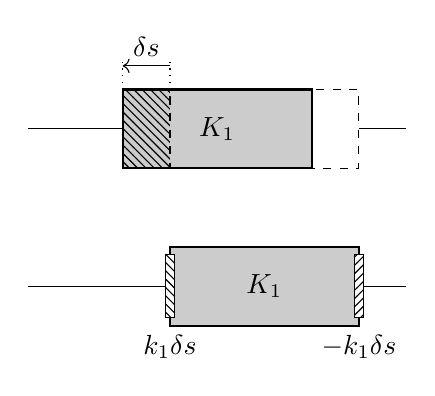
\begin{tikzpicture}[x=1.2cm]
	%		\draw (-4,0) -- (-1,0);
	%		\draw (1,0) -- (4,0);
	%		\draw[fill=black!20!white] (-.5,-.5) rectangle (1,.5);
	%		\filldraw[fill=white, draw=black, dashed] (1,-.5) rectangle (1.5,.5);
	%		\draw[pattern=north west lines, pattern color=black!20!white] (-1,-.5) rectangle (-.5,.5);
	%		\draw[black] (-1,-.5) rectangle (1,.5);
	
	\draw (-2,0) -- (-1,0);
	\draw (1,0) -- (2,0);
	
	\filldraw[fill=white, draw=black, dashed] (1,-.5) rectangle (1.5,.5);
	\fill[white!80!black] (-1,-.5) rectangle (1,.5);
	\node at (0.0,0) {$ K_1 $};
	\draw[pattern=north west lines, draw=none]  (-1,-.5) rectangle (-.5,.5);
	\draw[dashed] (-1,-.5) rectangle (-.5,.5);
	\draw[black,thick] (-1,-.5) rectangle (1,.5);
	
	\draw[->] (-.5, .8) -- (-1, .8);
	\draw[dotted] (-.5,.5) -- (-.5, .9);
	\draw[dotted] (-1,.5) -- (-1, .9);
    \node[above] at (-.75, .8) {$ \delta s $};
    \begin{scope}[shift={(0,-2)}]
	\draw (-2, 0) -- (-.5,0);
	\draw (1.5,0) --(2,0);
	%\draw (-.65,0) --(-.5,0);
	%\draw (1.0, 0) -- (1.15, 0);
	
	\filldraw[draw=black, thick, fill=white!80!black] (-.5,-.5) rectangle (1.5,.5);
	\node at (0.5,0) {$ K_1 $};
	\fill[white] (-.55, -.4) rectangle (-.45,.4);		
	\draw[pattern=north west lines] (-.55, -.4) rectangle (-.45,.4);
	
	\fill[white] (1.45, -.4) rectangle (1.55,.4);
	\draw[pattern=north east lines] (1.45, -.4) rectangle (1.55,.4);
	
	\node[below] at (-.5,-.5) {$k_1\delta s $};
    \node[below] at (1.5,-.5) {$- k_1\delta s  $};
    \end{scope}
	\end{tikzpicture}
\end{document}